\documentclass[10pt, a4paper,spanish]{article}
\usepackage[utf8]{inputenc}

\usepackage{lipsum} % Package to generate dummy text throughout this template
\usepackage{varwidth}
\usepackage{graphicx}

\usepackage[T1]{fontenc} % Use 8-bit encoding that has 256 glyphs
\usepackage{microtype} % Slightly tweak font spacing for aesthetics

\usepackage[hmarginratio=1:1,top=32mm,columnsep=20pt]{geometry} % Document margins
\usepackage{multicol} % Used for the two-column layout of the document
\usepackage[hang, small,labelfont=bf,up,textfont=it,up]{caption} % Custom captions under/above floats in tables or figures
\usepackage{booktabs} % Horizontal rules in tables
\usepackage{float} % Required for tables and figures in the multi-column environment - they need to be placed in specific locations with the [H] (e.g. \begin{table}[H])
\usepackage{hyperref} % For hyperlinks in the PDF

\usepackage{lettrine} % The lettrine is the first enlarged letter at the beginning of the text
\usepackage{paralist} % Used for the compactitem environment which makes bullet points with less space between them

\usepackage{abstract} % Allows abstract customization
\renewcommand{\abstractnamefont}{\normalfont\bfseries} % Set the "Abstract" text to bold
\renewcommand{\abstracttextfont}{\normalfont\small\itshape} % Set the abstract itself to small italic text

\usepackage{titlesec} % Allows customization of titles
\renewcommand\thesection{\Roman{section}} % Roman numerals for the sections
\renewcommand\thesubsection{\Roman{subsection}} % Roman numerals for subsections
\titleformat{\section}[block]{\large\scshape\centering}{\thesection.}{1em}{} % Change the look of the section titles
\titleformat{\subsection}[block]{\large}{\thesubsection.}{1em}{} % Change the look of the section titles

\usepackage{fancyhdr} % Headers and footers
\pagestyle{fancy} % All pages have headers and footers
\fancyhead{} % Blank out the default header
\fancyfoot{} % Blank out the default footer
\fancyhead[C]{Sergio García Prado $\bullet$ Febrero 2016 $\bullet$ Investigación de Operaciones} % Custom header text
\fancyfoot[RO,LE]{\thepage} % Custom footer text

%----------------------------------------------------------------------------------------
%	TITLE SECTION
%----------------------------------------------------------------------------------------

\title{\vspace{-15mm}\fontsize{24pt}{10pt}\selectfont\textbf{Investigación de Operaciones}} % Article title

\author{
\large
\textsc{Sergio García Prado}\\[2mm] % Your name
\normalsize Universidad de Valladolid \\ % Your institution
\vspace{-5mm}
}
\date{}

%----------------------------------------------------------------------------------------

\begin{document}

	\maketitle % Insert title

	\thispagestyle{fancy} % All pages have headers and footers

%----------------------------------------------------------------------------------------
%	ABSTRACT
%----------------------------------------------------------------------------------------

	\begin{abstract}
		\noindent Investigación de Operaciones 
	\end{abstract}

	\section{Orígenes}
	
		\paragraph{}
		Cuando comenzó la Segunda Guerra Mundial, había un pequeño grupo de investigadores militares, encabezados por A. P. Rowe, interesados en el uso militar de una técnica conocida como radioubicación (o radiolocalización), que desarrollaron científicos civiles. Algunos historiadores consideran que esta investigación es el punto inicial de la investigación de operaciones. Otros creen que los estudios que tienen las características del trabajo de investigación de operaciones aparecieron posteriormente. Algunos consideran que su comienzo está en el análisis y solución del bloqueo naval de Siracusa que Arquímedes presentó al tirano de esa ciudad, en el siglo III A.C. F. W. Lanchester, en Inglaterra, justo antes de la primera guerra mundial, desarrolló relaciones matemáticas sobre la potencia balística de las fuerzas opositoras que, si se resolvían tomando en cuenta el tiempo, podían determinar el resultado de un encuentro militar. Thomas Alva Edison también realizó estudios de guerra antisubmarina. Ni los estudios de Lanchester ni los de Edison tuvieron un impacto inmediato; junto con los de Arquímedes, constituyen viejos ejemplos del empleo de científicos para determinar la decisión óptima en las guerras, optimizando los ataques. \cite{wikipedia_IO}
		
		\paragraph{}
		En agosto de 1940 se organizó un grupo de 20 investigadores, bajo la dirección de P. M. S. Blackett, de la Universidad de Mánchester, para estudiar el uso de un nuevo sistema antiaéreo controlado por radar. Se conoció al grupo de investigación como “el Circo de Blackett”, nombre que no parece desatinado a la luz de sus antecedentes y orígenes diversos. El grupo estaba formado por tres fisiólogos, dos fisicomatemáticos, un astrofísico, un oficial del ejército, un topógrafo, un físico general y dos matemáticos. Generalmente se acepta que la formación de este grupo constituye el inicio de la investigación de operaciones. \cite{wikipedia_IO}
	
		\paragraph{}
		Al terminar la guerra, el éxito de la IO en las actividades bélicas generó gran interés debido a las posibilidades de aplicarla en un ámbito distinto al militar. Una vez que la explosión industrial posterior a la guerra siguió su curso, los problemas provocados por el aumento de la complejidad y la especialización de las organizaciones pasaron de nuevo al primer plano. Entonces comenzó a ser evidente para un gran número de personas, entre ellas los consultores industriales que habían trabajado con o para los equipos de IO durante la guerra, que estos problemas eran en esencia los mismos que los que debían enfrentar los militares pero en un contexto diferente. Al inicio de la década de los años cincuenta, estos visionarios introdujeron el uso de la investigación de operaciones en una serie de organizaciones industriales, de negocios y del gobierno. Desde entonces, se ha desarrollado con rapidez. \cite{hillier_lieberman_IO}
		
		\paragraph{}
		Un factor que dio gran impulso al desarrollo de este campo fue la revolución de las computadoras. El manejo eficaz de los complejos problemas inherentes a la IO casi siempre requiere un gran número de cálculos. Realizarlos de forma manual puede resultar casi imposible, por lo cual el desarrollo de la computadora electrónica digital, con su capacidad para hacer cálculos aritméticos, miles o tal vez millones de veces más rápido que los seres humanos, fue una gran ayuda para esta disciplina.	\cite{hillier_lieberman_IO}
		
		\begin{figure}[H]
				\centering
				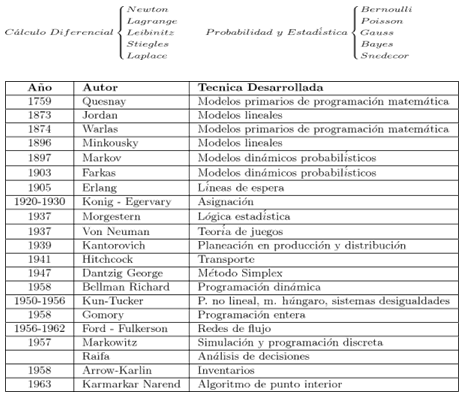
\includegraphics[width=120mm]{res/desarrollo-historico-de-la-investigacion-de-operaciones.png}
				\caption{Evolución histórica de la Investigación Operativa \protect\cite{hillier_lieberman_IO}} 
			\end{figure}
		
			
	\section{Naturaleza}
		\paragraph{}
		Investigación de Operaciones
			
	\section{Influencia}
		\paragraph{}
		Investigación de Operaciones
			
	\section{Etapas del estudio}
		\paragraph{}
		Investigación de Operaciones
					

%----------------------------------------------------------------------------------------
%	Bibliographic references
%----------------------------------------------------------------------------------------
	\begin{thebibliography}{9}
	
		\bibitem{wikipedia_IO} 
		Wikipedia. Investigación de Operaciones. \url{https://es.wikipedia.org/wiki/Investigación_de_operaciones}
		
		\bibitem{hillier_lieberman_IO} 
		Hillier / Lieberman. Introducción a la Investigacion de Operaciones.
		
		\bibitem{gestiopolis_IO_history}
		Gestiopolis. Desarrollo histórico de la investigación de operaciones. \url{http://www.gestiopolis.com/desarrollo-historico-de-la-investigacion-de-operaciones/}

		
	\end{thebibliography}

\end{document}
